\chapter{Introduction: Earth Observation and Deep Learning}
\label{ch:intro}

\chapmeta{Beginner}{$\sim$4\,h (2\,h theory + 2\,h practical)}{EuroSAT RGB (torchgeo, $\sim$90\,MB)}

\begin{objbox}
\begin{itemize}[leftmargin=1.2em,nosep]
  \item Understand what satellite imagery is and why it matters for AI.
  \item Load and visualise multi-band GeoTIFF files with \texttt{rasterio}.
  \item Understand spectral bands, spatial resolution, and coordinate reference systems (CRS).
  \item Explore the structure of the EuroSAT benchmark dataset.
  \item Build intuition for why CNNs --- not per-pixel classifiers --- extract land-use information.
\end{itemize}
\end{objbox}

\section{What is Earth Observation?}

Earth Observation (EO) is the systematic collection of information about the
Earth's physical, chemical and biological systems using remote sensors, chiefly
satellites. Unlike a consumer camera, an EO sensor does not produce a
``photograph''; it measures the intensity of electromagnetic radiation
reflected or emitted by the surface within a set of narrow wavelength intervals
called \emph{spectral bands}. Each band is itself a grey-scale image, so a
single acquisition is a stack of co-registered images --- a tensor of shape
$(C, H, W)$ where $C$ is the number of bands. This structural identity with the
input a CNN expects is the reason deep learning transferred so naturally to
remote sensing.

Four properties characterise any EO sensor and constrain the models we build on
top of it:
\begin{description}[leftmargin=1.6em,style=nextline]
  \item[Spatial resolution] the ground area covered by one pixel (the
  ground-sampling distance, GSD). Sentinel-2 is 10--60\,m; WorldView-3 reaches
  0.3\,m.
  \item[Spectral resolution] the number and width of the bands. More bands
  reveal more about surface chemistry (e.g.\ chlorophyll, moisture).
  \item[Temporal resolution] the revisit period. Sentinel-2 revisits every
  $\sim$5 days, enabling change-detection and time-series tasks.
  \item[Radiometric resolution] the bit depth of the measurement (Sentinel-2
  stores 12-bit reflectance scaled to integers).
\end{description}

\begin{center}\small
\renewcommand{\arraystretch}{1.15}
\begin{tabular}{@{}lllll@{}}
\toprule
Satellite & Operator & Resolution & Revisit & Bands\\
\midrule
Sentinel-2 & ESA & 10--60\,m & 5\,days & 13\\
Landsat 8/9 & USGS/NASA & 30\,m & 16\,days & 11\\
WorldView-3 & Maxar & 0.3\,m & 1\,day & 29\\
Planet NICFI & Planet & 4.77\,m & daily & 4\\
\bottomrule
\end{tabular}
\end{center}

Resolution drives architecture. At 10\,m/px a single Sentinel-2 pixel covers a
tennis court, so individual buildings are sub-pixel; at 0.3\,m/px cars and tree
crowns are resolved. The size of the objects you care about, measured in
pixels, must fit inside the network's receptive field (Chapter~\ref{ch:conv}).

\section{Spectral bands: what satellites measure}

The single most important EO concept for a newcomer is that \emph{each band is
an image}, and different materials have characteristic \emph{spectral
signatures} --- reflectance as a function of wavelength. Figure~\ref{fig:spec}
shows idealised signatures for four land-cover types across the Sentinel-2
bands.

\begin{figure}[h]
\centering
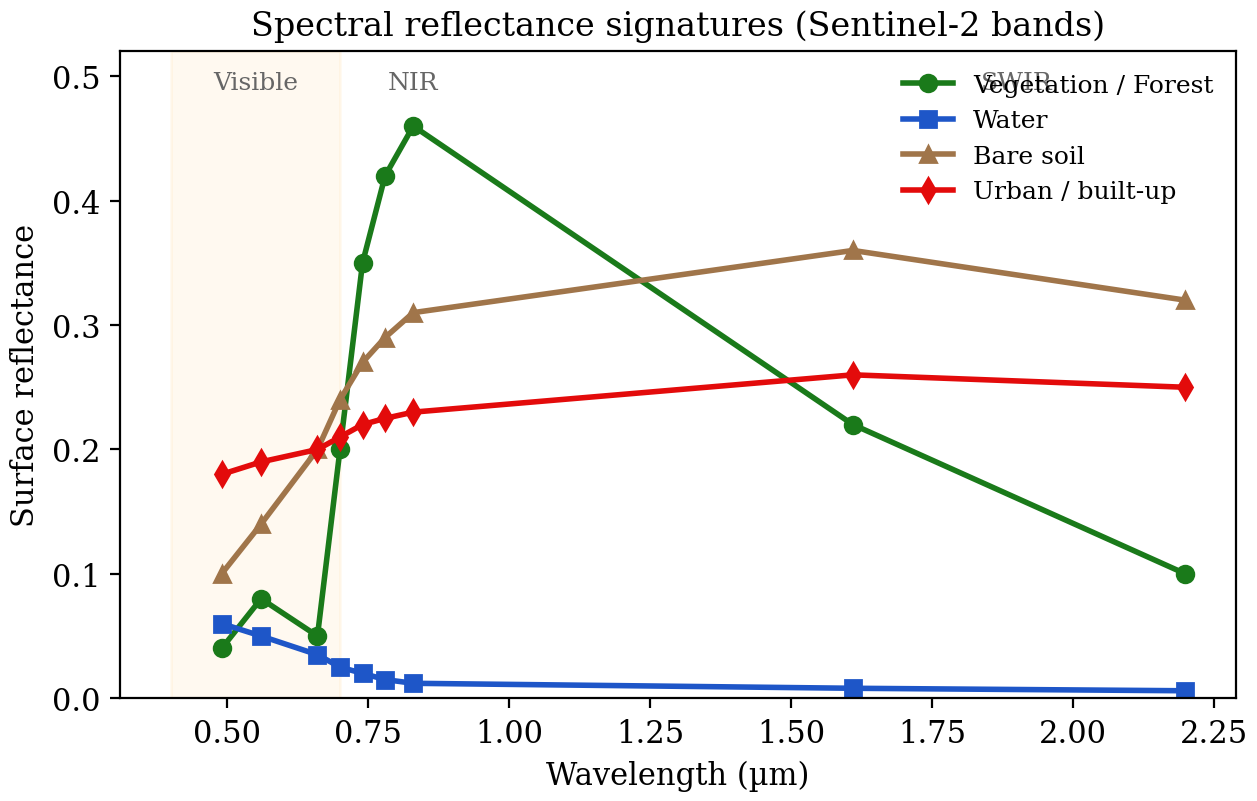
\includegraphics[width=0.82\linewidth]{figures/spectral_signatures.png}
\caption{Spectral reflectance signatures. Healthy vegetation reflects strongly
in the near-infrared (NIR, B08) and absorbs in the red (B04); water absorbs
almost everything beyond the visible; soil rises gently toward the SWIR. These
contrasts are exactly what spectral indices and CNNs exploit.}
\label{fig:spec}
\end{figure}

The vegetation ``red edge'' --- the steep rise between B04 (red) and B08 (NIR)
--- underlies the most famous remote-sensing index, the Normalised Difference
Vegetation Index:
\begin{equation}
\mathrm{NDVI} = \frac{\rho_\mathrm{NIR}-\rho_\mathrm{Red}}{\rho_\mathrm{NIR}+\rho_\mathrm{Red}}
= \frac{\mathrm{B08}-\mathrm{B04}}{\mathrm{B08}+\mathrm{B04}} \in [-1,1].
\label{eq:ndvi}
\end{equation}
Dense vegetation gives $\mathrm{NDVI}\gtrsim 0.6$; water gives negative values.
We will compute indices like this in Chapter~\ref{ch:preproc} and feed them as
extra channels to networks.

\begin{notebox}[Common pitfall]
Reflectance values are not 8-bit ``pixels''. Sentinel-2 Level-2A products store
bottom-of-atmosphere reflectance as integers (e.g.\ $0$--$10000$). Forgetting to
scale and normalise these before feeding a network is the single most frequent
beginner error (Chapter~\ref{ch:preproc}).
\end{notebox}

\section{Raster and vector data}

GIS data comes in two forms. \emph{Raster} data is a grid of pixels with a
geotransform mapping pixel $(row,col)$ to a world coordinate, plus a CRS
(coordinate reference system, e.g.\ EPSG:32633 for UTM zone 33N). Satellite
imagery and our prediction maps are rasters, read and written with
\texttt{rasterio}. \emph{Vector} data is geometry --- points, lines, polygons
--- stored in shapefiles or GeoJSON and manipulated with \texttt{geopandas};
building footprints and OpenStreetMap labels are vectors. Training a
segmentation model usually means \emph{rasterising} vector labels onto the same
grid as the imagery.

\section{The EuroSAT dataset}

EuroSAT (Helber et al., 2019) is the benchmark we use to learn the
classification machinery. It contains 27{,}000 Sentinel-2 patches of
$64\times64$ pixels, each labelled with one of ten land-use classes:
\textsf{AnnualCrop, Forest, HerbaceousVegetation, Highway, Industrial,
Pasture, PermanentCrop, Residential, River, SeaLake}. Two variants exist: RGB
(3 bands) and multispectral (13 bands). It is clean, balanced
($\sim$2000--3000 samples/class) and downloads in one line via
\texttt{torchgeo}, which makes it perfect for fast iteration --- but note that a
patch-level label teaches \emph{classification only}; it cannot teach the
spatial prediction we build toward later.

\section{Why CNNs, not per-pixel classifiers?}

Classical remote sensing classified each pixel independently from its spectral
vector using SVMs or random forests. This ignores \emph{spatial context}.
Consider the visual texture of land cover: forests have a rough, self-similar
canopy; urban areas show grid-like street patterns and high local heterogeneity;
water is smooth and homogeneous; agriculture shows regular field boundaries and
row striping. None of these are visible to a per-pixel method, because they live
in the \emph{neighbourhood} of a pixel, not in the pixel itself. A convolutional
network learns spatial filters that respond to exactly such patterns, and
stacks them into a hierarchy --- the subject of the next three chapters.

\begin{keybox}
\begin{itemize}[leftmargin=1.2em,nosep]
  \item Each spectral band is an image; an acquisition is a $(C,H,W)$ tensor.
  \item Spectral signatures distinguish materials; indices such as NDVI
  (Eq.~\ref{eq:ndvi}) summarise them.
  \item Reflectance must be scaled and normalised before training.
  \item Raster (pixels + CRS) vs vector (geometry); labels are often rasterised.
  \item CNNs learn \emph{spatial} patterns that per-pixel classifiers miss.
\end{itemize}
\end{keybox}

\begin{practbox}
Notebook: \nbpath{notebooks/chapter\_01\_intro\_eo\_dl/01\_practical\_eo\_data\_exploration.ipynb}.
\begin{enumerate}[leftmargin=1.4em,nosep]
  \item Run the Colab/environment setup cell; confirm \texttt{DEVICE} and
  \texttt{FAST\_MODE} are detected.
  \item Download EuroSAT RGB via \texttt{torchgeo} and visualise one sample per
  class in a $2\times5$ grid.
  \item Inspect the class distribution as a bar chart; confirm the dataset is
  near-balanced.
  \item Read a multi-band GeoTIFF with \texttt{rasterio}; print its shape, dtype,
  CRS and geotransform; render a true-colour composite from B04/B03/B02.
  \item Compute and display NDVI for a vegetated and a water sample.
\end{enumerate}
A representative skeleton for reading a scene and computing an index:
\begin{lstlisting}
import rasterio, numpy as np
with rasterio.open(path) as src:
    img = src.read().astype("float32")   # (C, H, W)
    print(img.shape, src.crs, src.transform)
red, nir = img[3], img[7]                  # B04, B08 (0-indexed)
ndvi = (nir - red) / (nir + red + 1e-6)
\end{lstlisting}
\end{practbox}

\begin{exbox}
\textbf{1.1 Channel statistics.} Over the EuroSAT test split, compute the per-channel
mean and standard deviation. Tabulate them --- these become your normalization
constants in Chapter~\ref{ch:classif}.\\[2pt]
\textbf{1.2 Spectral profiles.} For five random samples from each class, plot the
mean reflectance vs band number. Verify water has near-zero NIR/SWIR and forest
has high NIR.\\[2pt]
\textbf{1.3 NDVI thresholding.} Using EuroSAT-MS, compute NDVI for three
\textsf{Forest} and three \textsf{SeaLake} samples; find a threshold separating
them.\\[2pt]
\textbf{Mini-project.} Write \texttt{describe\_sample(idx)} that prints the class
name, RGB and NIR means, and shows the RGB image beside an NDVI heatmap; run it
on five samples.
\end{exbox}
